\chapter{Additional Tests}
\section{Effect of the BHA Size}
A sensitivity test was conducted to assess the impact of the BHA size on drill string vibration. For these simulations, exaggerated sizes of the BHA components were employed. The cases were based on Test Case 4b but different BHAs were used. Test Case 4b\_A1, Test Case 4b\_A2, and Test Case 4b\_A3 were run with the BHA's components outer diameter doubled, triple the length of the BHA, and both, respectively. \tablename~\ref{table_sensitivity_size_4b_input} summarizes the BHA properties for the tests.  The complete set of parameters are shown in \tablename~\ref{table_Inclinedwell_4b_A1_input}, \ref{table_Inclinedwell_4b_A2_input}, and~\ref{table_Inclinedwell_4b_A3_input} for Test Case 4b\_A1, Test Case 4b\_A2, and Test Case 4b\_A3, respectively.
\begin{table}
	\centering
	\begin{tabular}{|c|c|c|c|c|c|}
		\hline
        \tablecolumnheadervlinesone{Parameter} & \tablecolumnheadervlinestwo{Test Case 4b} & \tablecolumnheadervlinestwo{Test Case 4b\_A1} & \tablecolumnheadervlinestwo{Test Case 4b\_A2} & \tablecolumnheadervlinestwo{Test Case 4b\_A3} \\
		\hline
		$OD_{HWDP}$ & 0.1143 $m$ & 0.2286 $m$ & 0.1143 $m$ & 0.2286 $m$ \\
		\hline
		$ID_{HWDP}$ & 0.0635 $m$ & 0.0635 $m$ & 0.0635 $m$ & 0.0635 $m$ \\
		\hline
		$L_{HWDP}$ & 18.30 $m$ & 18.30 $m$ & 54.6 $m$ & 54.6 $m$ \\
		\hline
		$OD_{DC}$ & 0.1524 $m$ & 0.3048 $m$ & 0.1524 $m$ & 0.3048 $m$ \\
		\hline
		$ID_{DC}$ & 0.0508 $m$ & 0.0508 $m$ & 0.0508 $m$ & 0.0508 $m$ \\
		\hline
		$L_{DC}$ & 82.30 $m$ & 82.30 $m$ & 249.6 $m$ & 249.6 $m$ \\
		\hline
	\end{tabular}
	\caption[Comparison of the input parameters used for the BHA size tests.]{Comparison of the input parameters used for the BHA size tests.  The tests were based on Test Case 4b.}
	\label{table_sensitivity_size_4b_input}
\end{table}
\begin{table}
	\centering
	\begin{testcasetable}
		$\rho$ & 490.6 $lb/ft^3$ & 7850 $kg/m^3$ & Drill pipe density \\
		\hline
		$G_{DP}$ & 1.67$\cdot$10$^{9}$ $lbf/ft^2$ & 7.99$\cdot$10$^{10}$ $Pa$  & Shear modulus \\
		\hline
		$OD_{DP}$ & 5.88 $in$ & 0.15 $m$ & Drill pipe outer diameter \\
		\hline
		$ID_{DP}$ & 5.00 $in$ & 0.127 $m$ & Drill pipe inner diameter  \\
		\hline
		$OD_{HWDP}$ & 9.00 $in$ & 0.2286 $m$ & Heavy weight drill pipe outer diameter \\
		\hline
		$ID_{HWDP}$ & 2.50 $in$ & 0.0635 $m$ & Heavy weight drill pipe inner diameter \\
		\hline
		$L_{HWDP}$ & 60.0 $ft$ & 18.30 $m$ & Length of heavy weight drill pipe \\
		\hline
		$OD_{DC}$ & 12.0 $in$ & 0.3048 $m$ & Drill collars outer diameter \\
		\hline
		$ID_{DC}$ & 2.00 $in$ & 0.0508 $m$ & Drill collars inner diameter \\
		\hline
		$L_{DC}$ & 270.0 $ft$ & 82.30 $m$ & Length of drill collars \\
		\hline
		$\mu_{s}$ & 0.5 & 0.5 & Static friction factor \\
		\hline
		$\mu_{d}$ & 0.25 & 0.25 & Dynamic friction factor \\
		\hline
		$w_c$ & 10 $RPM$ & 10 $RPM$ & Friction critical velocity \\
		\hline
		$\theta$ & 60$^{\circ}$ & 60$^{\circ}$ & Inclination \\
		\hline
		$KOP$ & 4921.3 $ft$ & 1500 $m$ & Kick off point \\
		\hline
		$EOB$ & 6889.8 $ft$ & 2100 $m$ & End of bend \\
		\hline
		$BD$ & 8202.1 $ft$ & 2500 $m$ & Bit depth \\
		\hline
		$MD$ & 13123.4 $ft$ & 4000 $m$ & Measured depth \\
		\hline
	\end{testcasetable}
	\caption[Input parameters for Test Case 4b\_A1]{Input parameters for Test Case 4b\_A1, a deviated well with BHA components and with different static and dynamic friction factors.}
	\label{table_Inclinedwell_4b_A1_input}
\end{table}
\begin{table}
	\centering
	\begin{testcasetable}
		$\rho$ & 490.6 $lb/ft^3$ & 7850 $kg/m^3$ & Drill pipe density \\
		\hline
		$G_{DP}$ & 1.67$\cdot$10$^{9}$ $lbf/ft^2$ & 7.99$\cdot$10$^{10}$ $Pa$  & Shear modulus \\
		\hline
		$OD_{DP}$ & 5.88 $in$ & 0.15 $m$ & Drill pipe outer diameter \\
		\hline
		$ID_{DP}$ & 5.00 $in$ & 0.127 $m$ & Drill pipe inner diameter  \\
		\hline
		$OD_{HWDP}$ & 4.50 $in$ & 0.1143 $m$ & Heavy weight drill pipe outer diameter \\
		\hline
		$ID_{HWDP}$ & 2.50 $in$ & 0.0635 $m$ & Heavy weight drill pipe inner diameter \\
		\hline
		$L_{HWDP}$ & 179.1 $ft$ & 54.6 $m$ & Length of heavy weight drill pipe \\
		\hline
		$OD_{DC}$ & 6.00 $in$ & 0.1524 $m$ & Drill collars outer diameter \\
		\hline
		$ID_{DC}$ & 2.00 $in$ & 0.0508 $m$ & Drill collars inner diameter \\
		\hline
		$L_{DC}$ & 818.9 $ft$ & 249.6 $m$ & Length of drill collars \\
		\hline
		$\mu_{s}$ & 0.5 & 0.5 & Static friction factor \\
		\hline
		$\mu_{d}$ & 0.25 & 0.25 & Dynamic friction factor \\
		\hline
		$w_c$ & 10 $RPM$ & 10 $RPM$ & Friction critical velocity \\
		\hline
		$\theta$ & 60$^{\circ}$ & 60$^{\circ}$ & Inclination \\
		\hline
		$KOP$ & 4921.3 $ft$ & 1500 $m$ & Kick off point \\
		\hline
		$EOB$ & 6889.8 $ft$ & 2100 $m$ & End of bend \\
		\hline
		$BD$ & 8202.1 $ft$ & 2500 $m$ & Bit depth \\
		\hline
		$MD$ & 13123.4 $ft$ & 4000 $m$ & Measured depth \\
		\hline
	\end{testcasetable}
	\caption[Input parameters for Test Case 4b\_A2]{Input parameters for Test Case 4\_A2b, a deviated well with BHA components and with different static and dynamic friction factors.}
	\label{table_Inclinedwell_4b_A2_input}
\end{table}
\begin{table}
	\centering
	\begin{testcasetable}
		$\rho$ & 490.6 $lb/ft^3$ & 7850 $kg/m^3$ & Drill pipe density \\
		\hline
		$G_{DP}$ & 1.67$\cdot$10$^{9}$ $lbf/ft^2$ & 7.99$\cdot$10$^{10}$ $Pa$  & Shear modulus \\
		\hline
		$OD_{DP}$ & 5.88 $in$ & 0.15 $m$ & Drill pipe outer diameter \\
		\hline
		$ID_{DP}$ & 5.00 $in$ & 0.127 $m$ & Drill pipe inner diameter  \\
		\hline
		$OD_{HWDP}$ & 9.00 $in$ & 0.2286 $m$ & Heavy weight drill pipe outer diameter \\
		\hline
		$ID_{HWDP}$ & 2.50 $in$ & 0.0635 $m$ & Heavy weight drill pipe inner diameter \\
		\hline
		$L_{HWDP}$ & 179.1 $ft$ & 54.6 $m$ & Length of heavy weight drill pipe \\
		\hline
		$OD_{DC}$ & 12.0 $in$ & 0.3048 $m$ & Drill collars outer diameter \\
		\hline
		$ID_{DC}$ & 2.00 $in$ & 0.0508 $m$ & Drill collars inner diameter \\
		\hline
		$L_{DC}$ & 818.9 $ft$ & 249.6 $m$ & Length of drill collars \\
		\hline
		$\mu_{s}$ & 0.5 & 0.5 & Static friction factor \\
		\hline
		$\mu_{d}$ & 0.25 & 0.25 & Dynamic friction factor \\
		\hline
		$w_c$ & 10 $RPM$ & 10 $RPM$ & Friction critical velocity \\
		\hline
		$\theta$ & 60$^{\circ}$ & 60$^{\circ}$ & Inclination \\
		\hline
		$KOP$ & 4921.3 $ft$ & 1500 $m$ & Kick off point \\
		\hline
		$EOB$ & 6889.8 $ft$ & 2100 $m$ & End of bend \\
		\hline
		$BD$ & 8202.1 $ft$ & 2500 $m$ & Bit depth \\
		\hline
		$MD$ & 13123.4 $ft$ & 4000 $m$ & Measured depth \\
		\hline
	\end{testcasetable}
	\caption[Input parameters for Test Case 4b\_A3]{Input parameters for Test Case 4b\_A3, a deviated well with BHA components and with different static and dynamic friction factors.}
	\label{table_Inclinedwell_4b_A3_input}
\end{table}

The results presented in \figurename{}s~\ref{figure_AS_BHA_size_effect_vel} and \ref{figure_AS_BHA_size_effect_td} demonstrate the influence of the BHA size on the angular velocity and torque, respectively. Increasing the diameter of the BHA increased the maximum torque and decreased the frequency.  The increase in BHA length also increased the torque and decreased the vibration frequency.  Combining both changes to create a larger diameter and longer BHA amplified the effects further.

The larger diameter BHA increased the mass.  Because the mass was largely concentrated at the end of the string, it did not significantly change the overall stiffness.  This appreciably decreased the frequency of vibration.  It also increased the torque.  The increased mass required a larger force to accelerate it.  In addition, as this is a deviated well case, the increased mass also increased the friction forces and required more torque overcome them.

Lengthening the BHA added mass and increased the stiffness.  The increased mass has all the same effects as mentioned in the previous paragraph.  It should be noted that the overall length of the drill string was held constant for these Test Cases.  Therefore, more of the stiffer BHA elements/sections were used and fewer of the softer drill pipe sections.  This increased the overall stiffness and decrease the frequency of vibration.  The added mass and increased stiffness offset each other in terms of the frequency effects.  By comparing the baseline and A2 tests in \figurename{}~\ref{figure_AS_BHA_size_effect_td}, it appears the mass affected the frequency more than the stiffness and the frequency decreased slightly. 
%It is observed that when the BHA length was increased (Test Case 4b versus Test Case 4b\_A2) a sudden increase in bit angular velocity occurred after the stick phase, while it originally occurred right before the stick phase. Moreover, the spikes of the bit velocity below 0 $RPM$ occurred when the BHA length was increased.

\begin{figure}
	\centering
	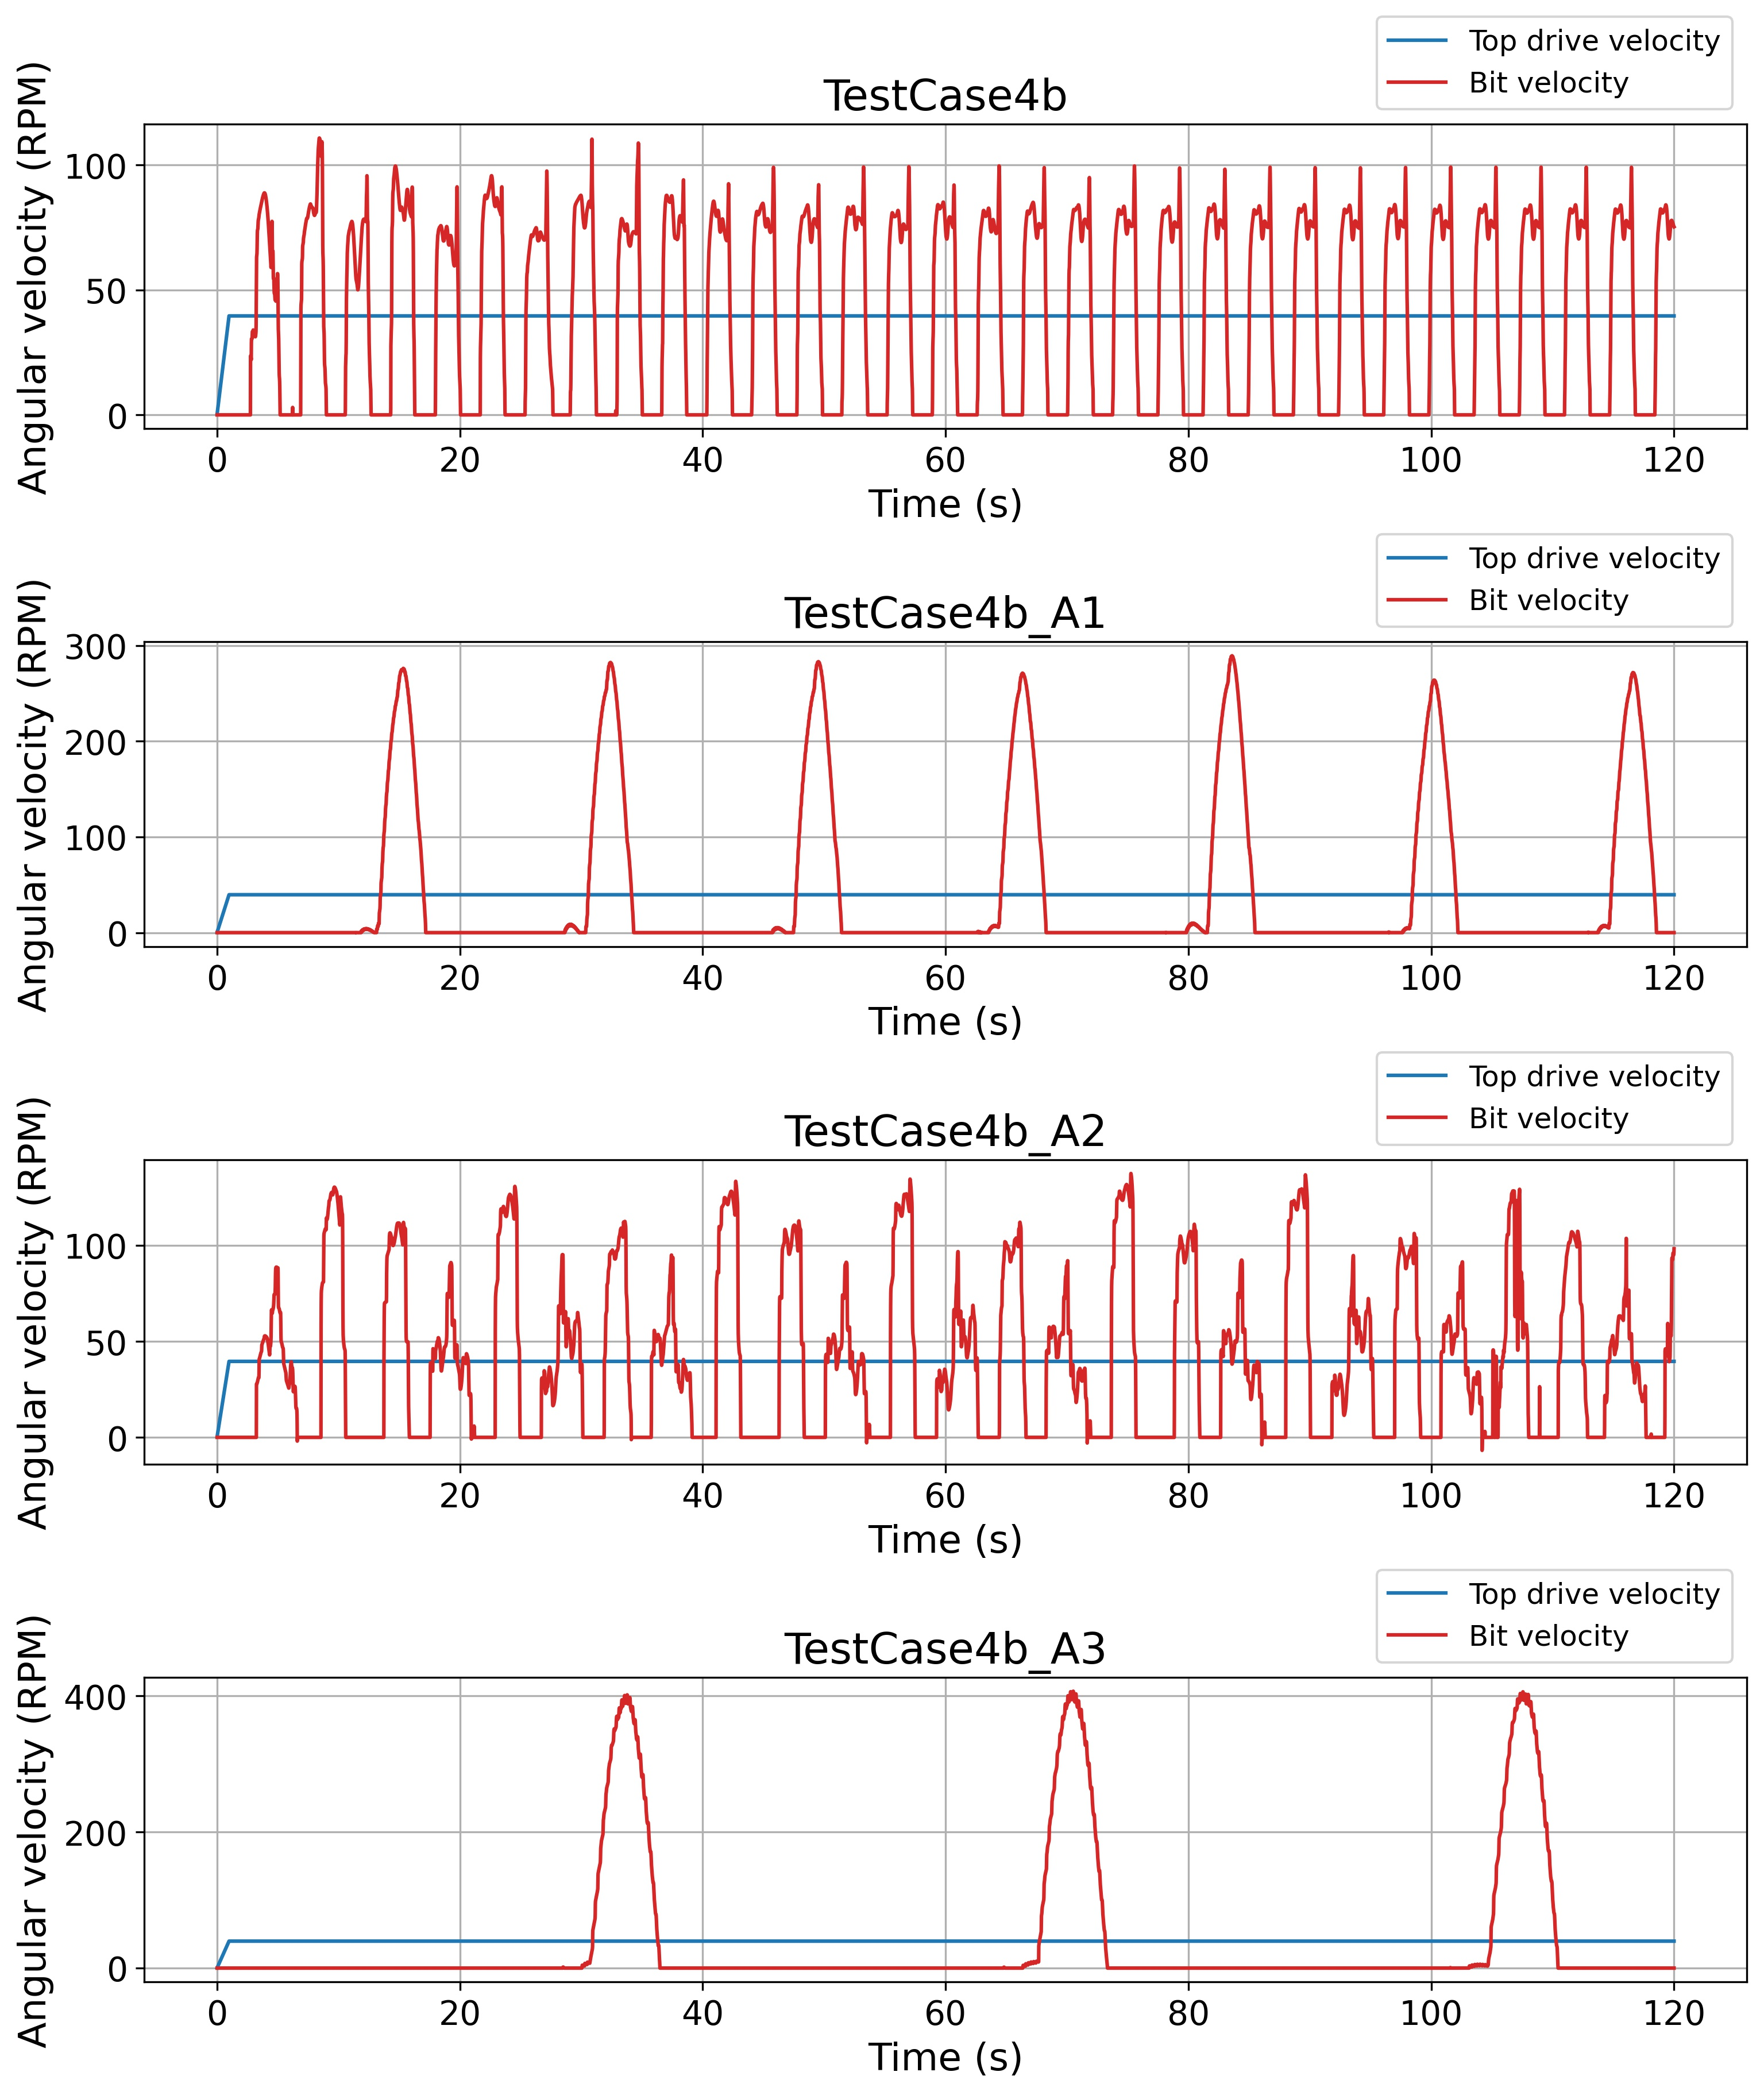
\includegraphics[width=\linewidth]{AS_size_effect_vel}
    \caption[Size effect of BHA components to angular velocity from A-S model]{Size effect of BHA components to angular velocity of bit from A-S model. The tests were conducted based on Test Case 4, where Test Case 4\_A1, Test Case 4\_A2 and Test Case 4\_A3 were simulated with doubled diameter, tripled length and both doubled diameter and tripled length of BHA components, respectively.}
	\label{figure_AS_BHA_size_effect_vel}
\end{figure}

\begin{figure}
	\centering
	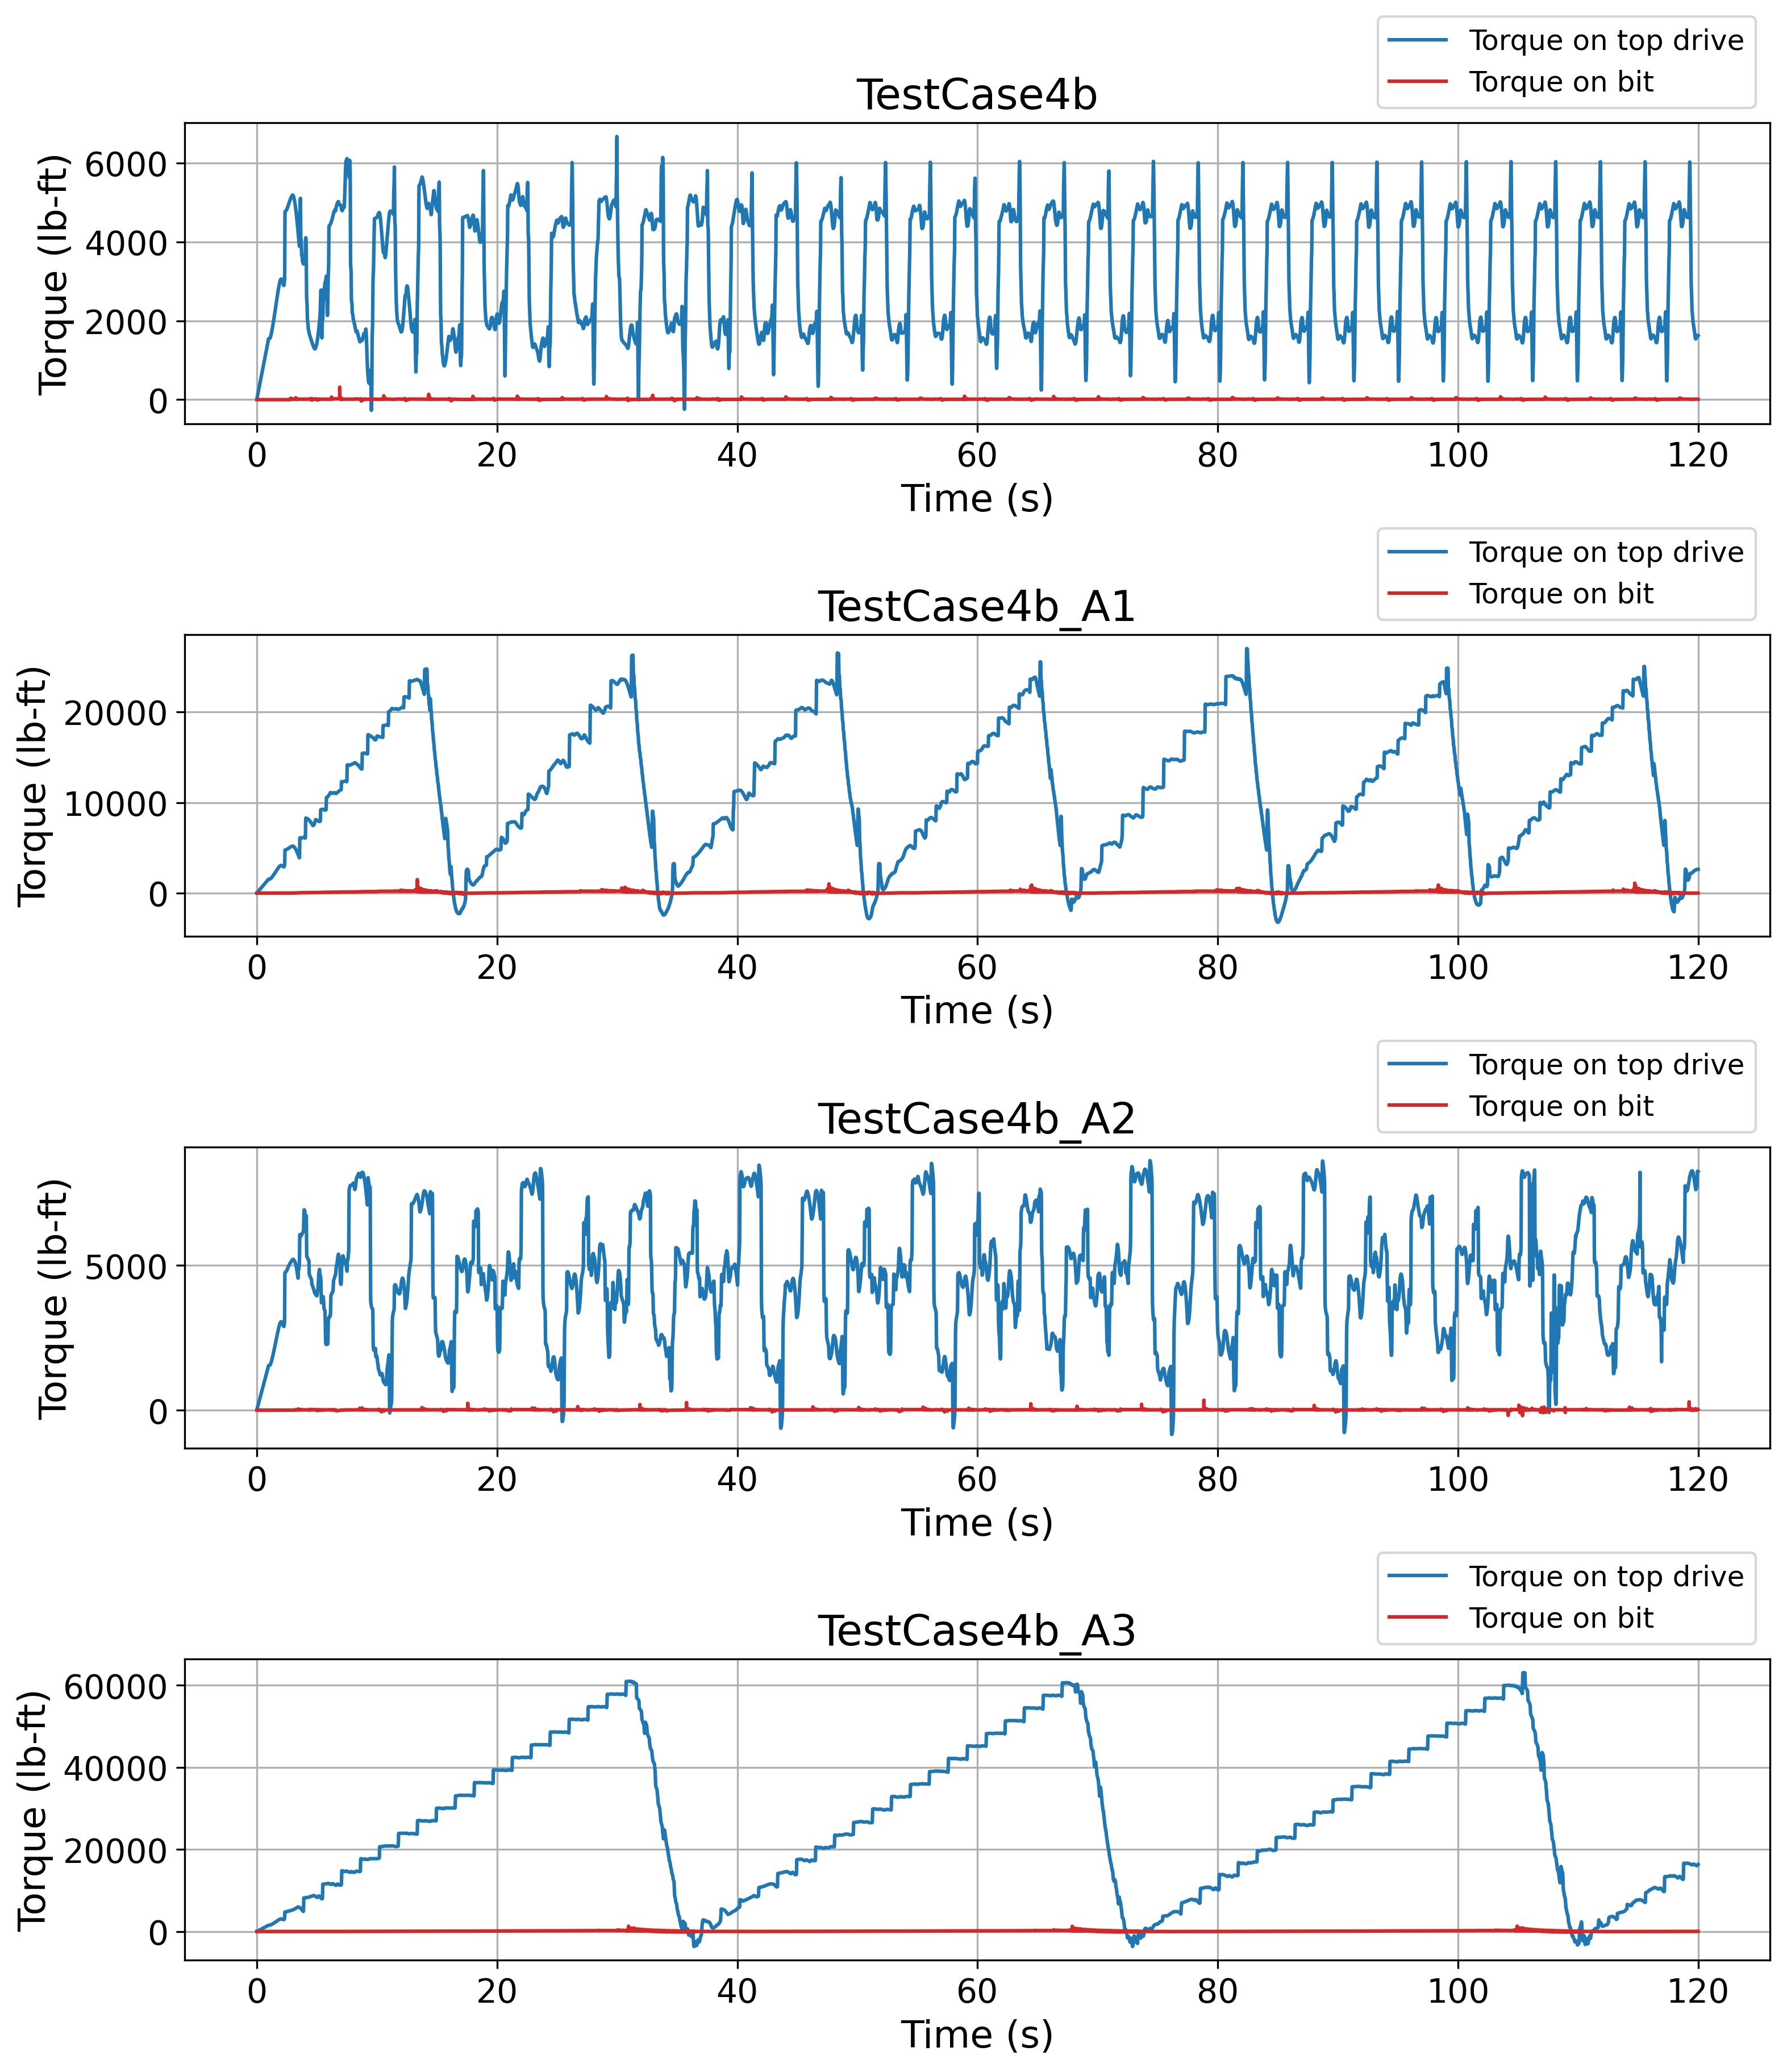
\includegraphics[width=\linewidth]{AS_size_effect_td}
    \caption[Size effect of BHA components to a torque from A-S model]{Size effect of BHA components to torque on top drive from A-S model. The tests were conducted based on Test Case 4, where Test Case 4\_A1, Test Case 4\_A2 and Test Case 4\_A3 were simulated with doubled diameter, tripled length and both doubled diameter and tripled length of BHA components, respectively.}
	\label{figure_AS_BHA_size_effect_td}
\end{figure}

%\section{Effect of Shear Modulus}

\section{Effect of Friction Model}
The influence of the friction model was assessed by implementing the Stribeck friction model inside the A-S model (Matlab ver.), which already included the Coulomb friction model. This analysis was conducted using Test Case 2. \figurename{}s~\ref{fig:friction_at_bit_coulomb} and \ref{fig:friction_at_bit_stribeck} illustrate the frictional force at the bit when the model was run with the Coulomb and Stribeck friction models, respectively.

With the Coulomb friction model, the friction jumps between the static and dynamic conditions.  Conversely, with the Stribeck model, the frictional force demonstrates a smoother trend.

\figurename{}s~\ref{figure_coloumb_coulomb} and~\ref{figure_coulomb_stribeck} present a comparison between the A-S and ExxonMobil models, incorporating both the Coulomb and Stribeck models in the A-S model. \figurename{}~\ref{figure_coloumb_coulomb} illustrates the A-S model with the Coulomb friction model, while \figurename{}~\ref{figure_coulomb_stribeck} depicts the A-S model with the Stribeck friction model. It is noteworthy that only the A-S model applied different friction models while ExxonMobil model only used the Stribeck friction model.

Test Case 2 has is a simple configuration; hence, the friction model did not exhibit a critical effect. However, a closer match between the A-S and ExxonMobil models was observed when the same friction model was applied. Additionally, fluctuations during the stick phase were only noticed when the Stribeck friction model was applied. It is expected that further studies involving more complex test cases could provide valuable insights into the impact of different friction models.

\begin{figure}
	\begin{minipage}[t]{\linewidth}
		\begin{minipage}[t]{\linewidth}
			\centering
			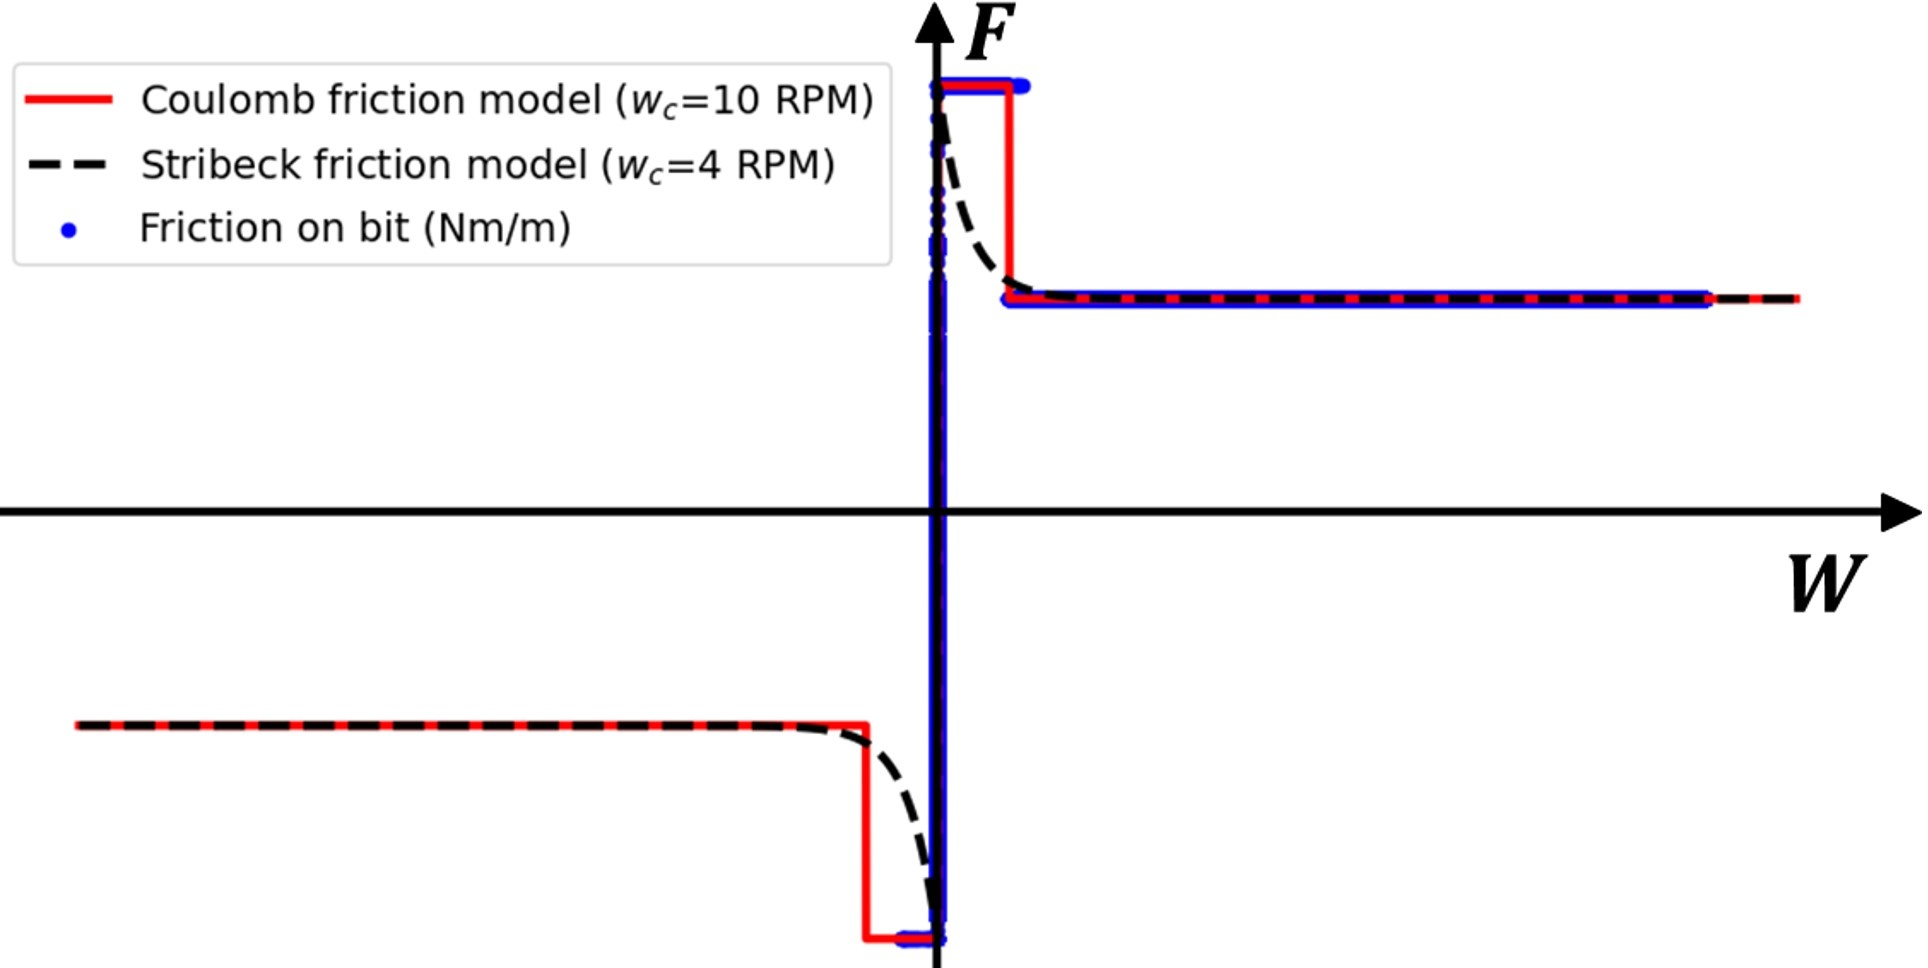
\includegraphics[width=0.6\linewidth]{friction_at_bit_coulomb_hysteresis}
            \subcaption{The friction force hysteresis from the A-S drill string model using a Coulomb friction model.  The calculated results are overlaid on top of both the Coulomb and Stribeck friction models for comparison.}
            \label{fig:friction_at_bit_coulomb_hysteresis}
		\end{minipage}
		\begin{minipage}[t]{\linewidth}
			\centering
			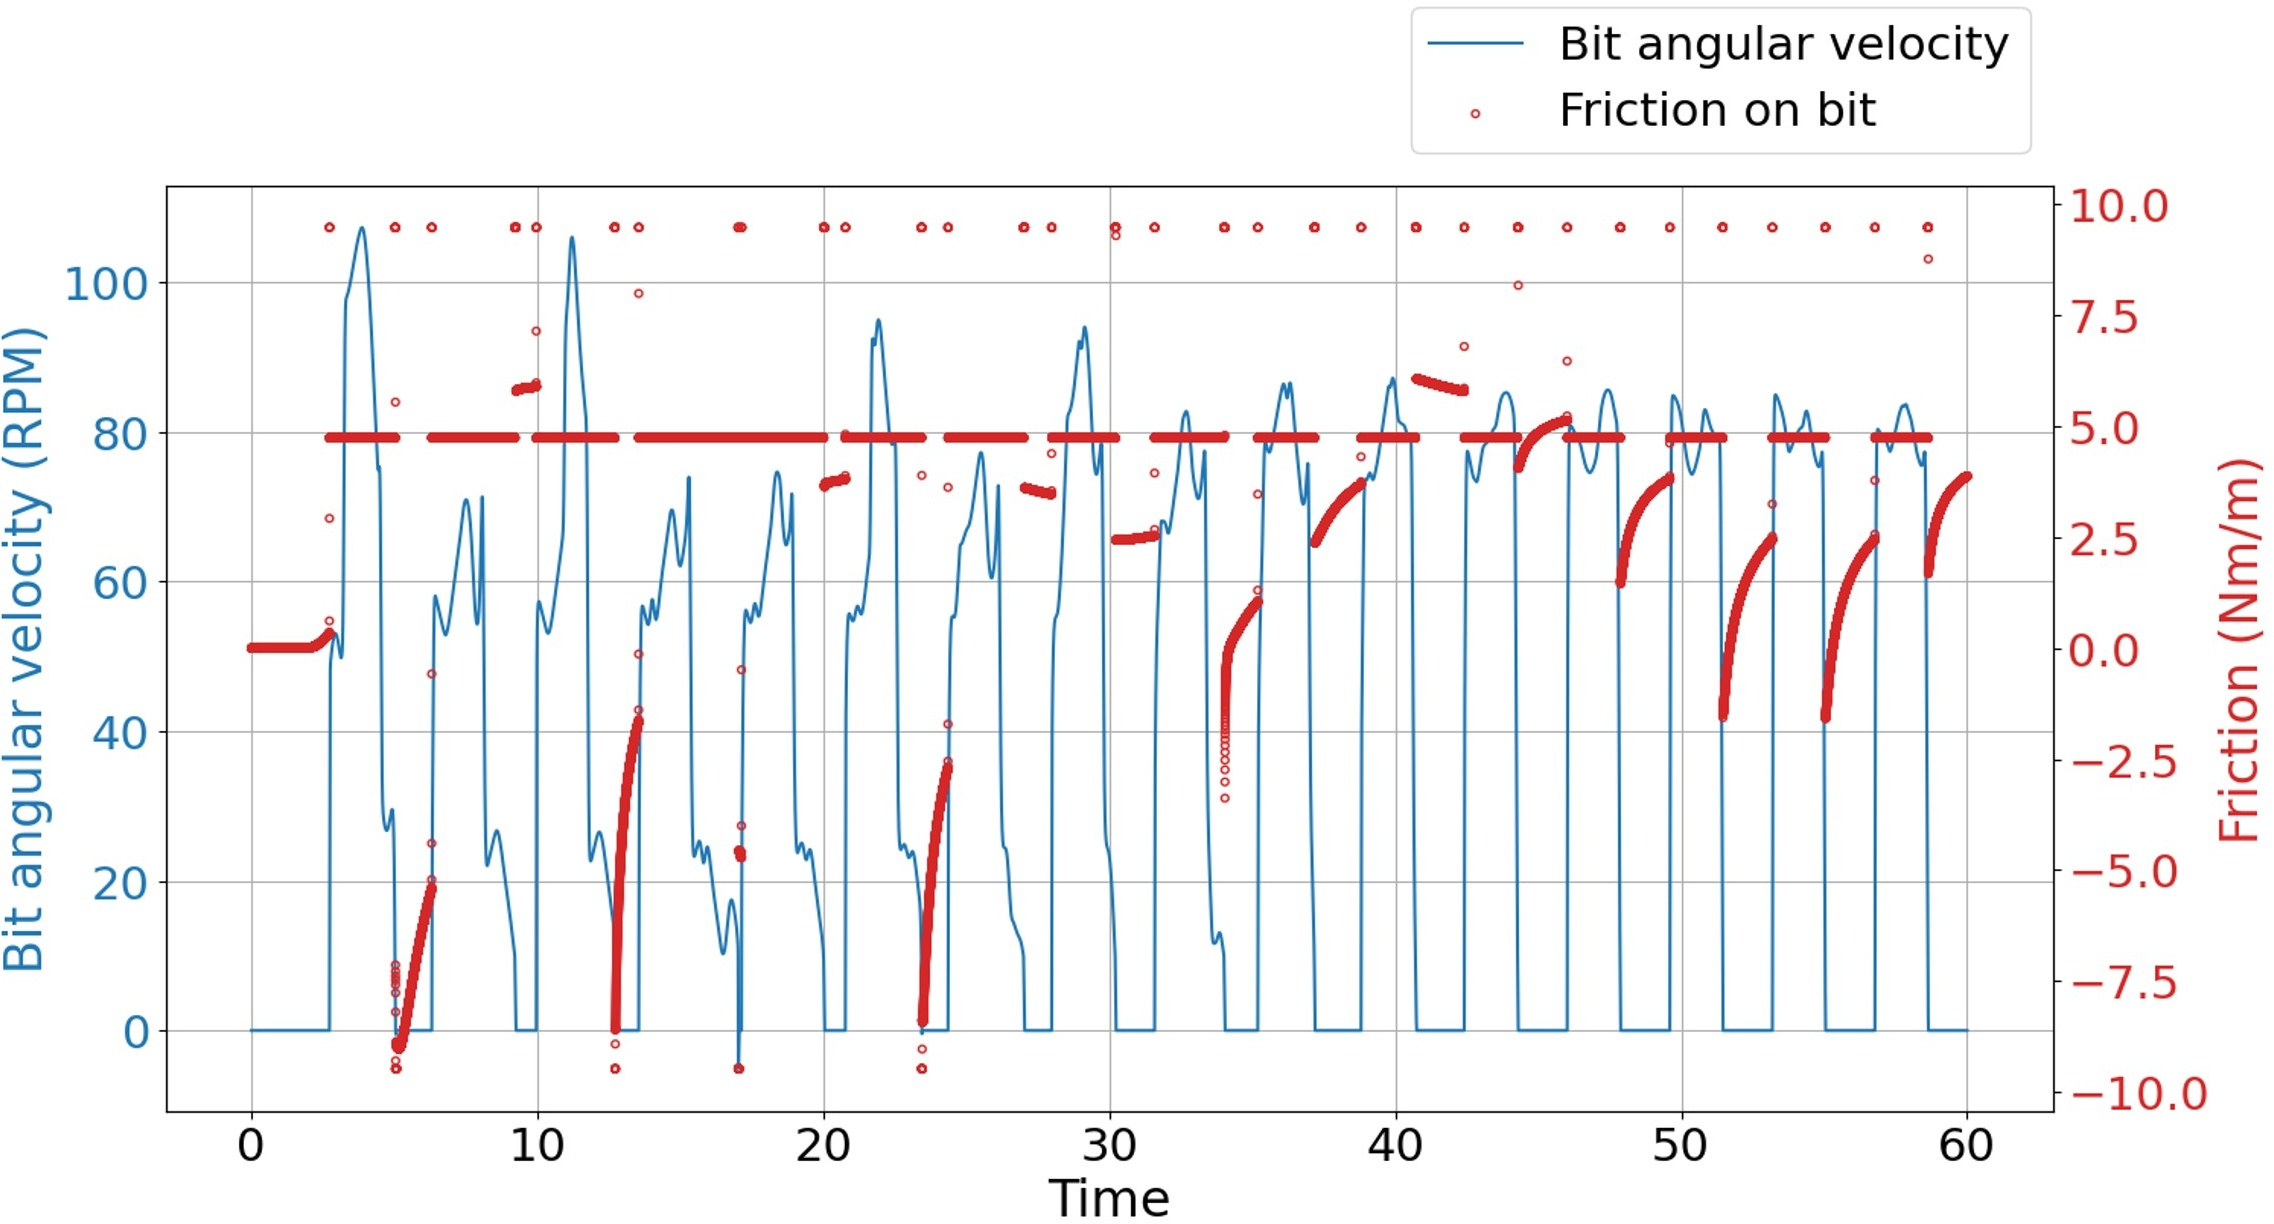
\includegraphics[width=0.85\linewidth]{friction_at_bit_coulomb_time}
			\subcaption{The frictional force at the bit and the angular velocity from the A-S drill string model using a Coulomb friction model.}
			\label{fig:friction_at_bit_coulomb_time}
		\end{minipage}
	\end{minipage}
    \caption[The friction forces from the A-S drill string model using a Coulomb friction model]{The friction forces from the A-S drill string model using a Coulomb friction model.  In~(\subref{fig:friction_at_bit_coulomb_hysteresis}), the calculated results are compared to be Coulomb and Stribeck friction models.  In~(\subref{fig:friction_at_bit_coulomb_time}), the calculated friction force is compared to the bit angular velocity.}
    \label{fig:friction_at_bit_coulomb}
\end{figure}

\begin{figure}
	\begin{minipage}[t]{\linewidth}
		\begin{minipage}[t]{\linewidth}
			\centering
			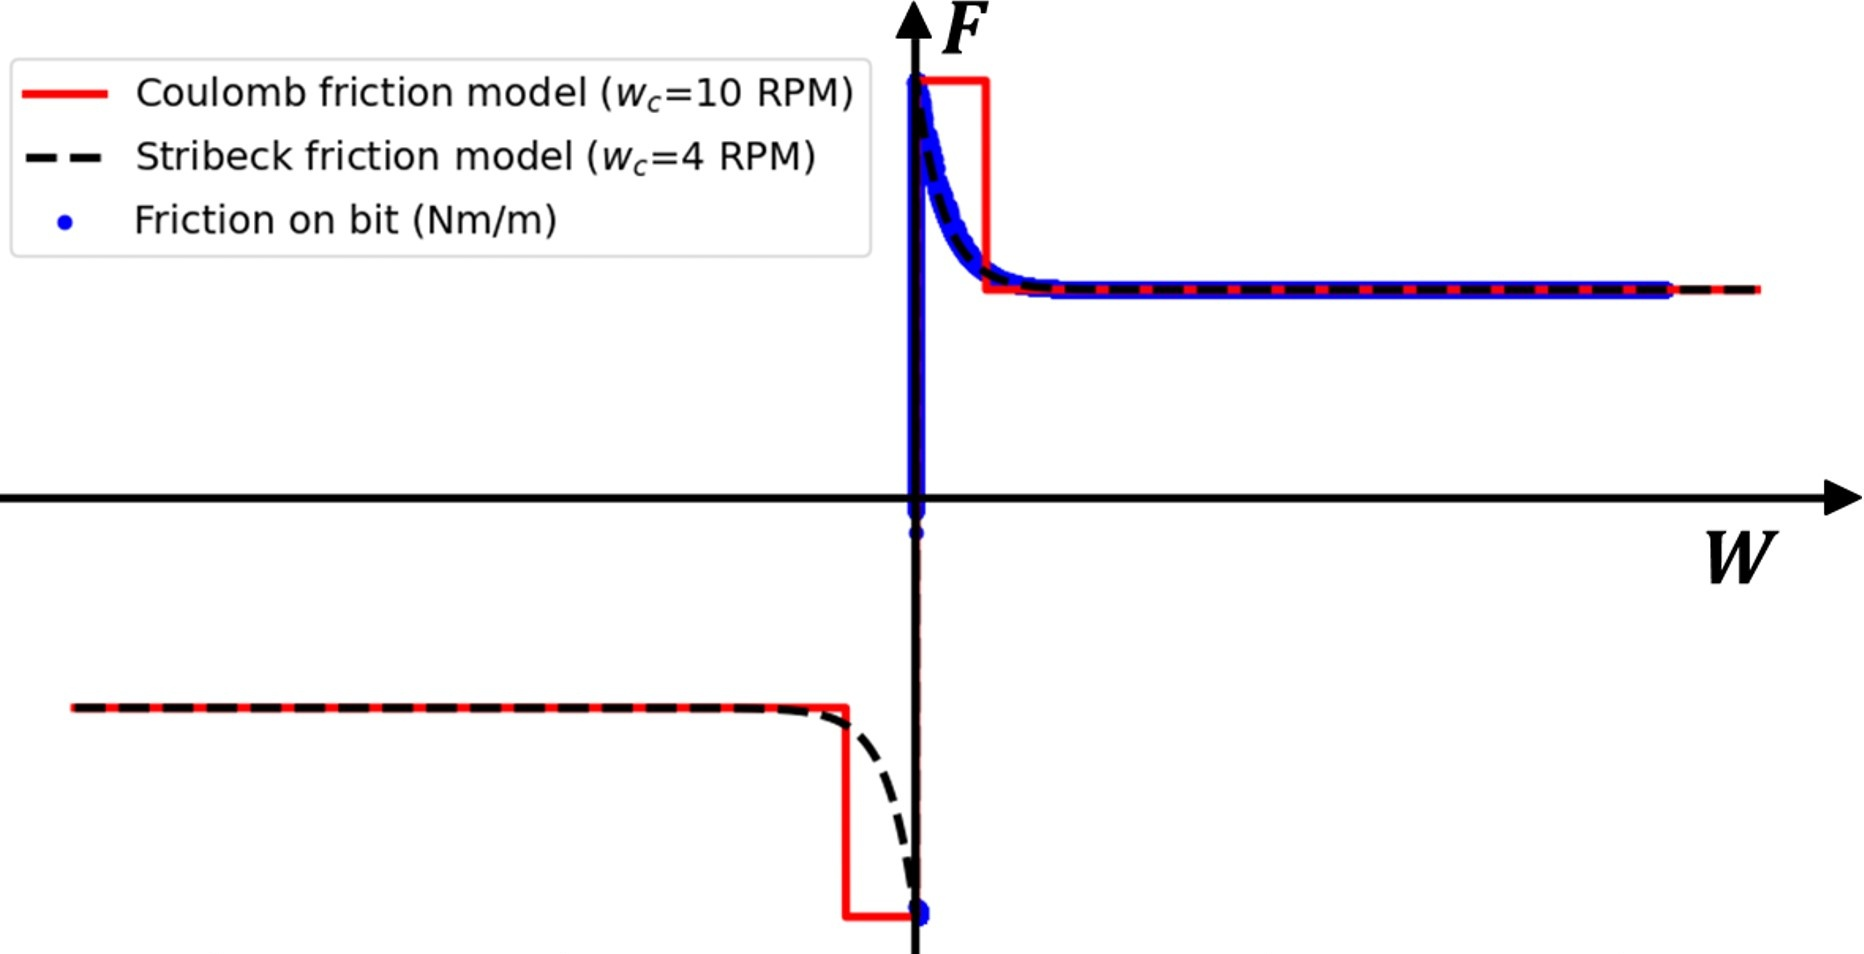
\includegraphics[width=0.6\linewidth]{friction_at_bit_stribeck_hysteresis}
            \subcaption{The friction force hysteresis from the A-S drill string model using a Stribeck friction model.  The calculated results are overlaid on top of both the Coulomb and Stribeck friction models for comparison.}
            \label{fig:friction_at_bit_stribeck_hysteresis}
		\end{minipage}
		\begin{minipage}[t]{\linewidth}
			\centering
			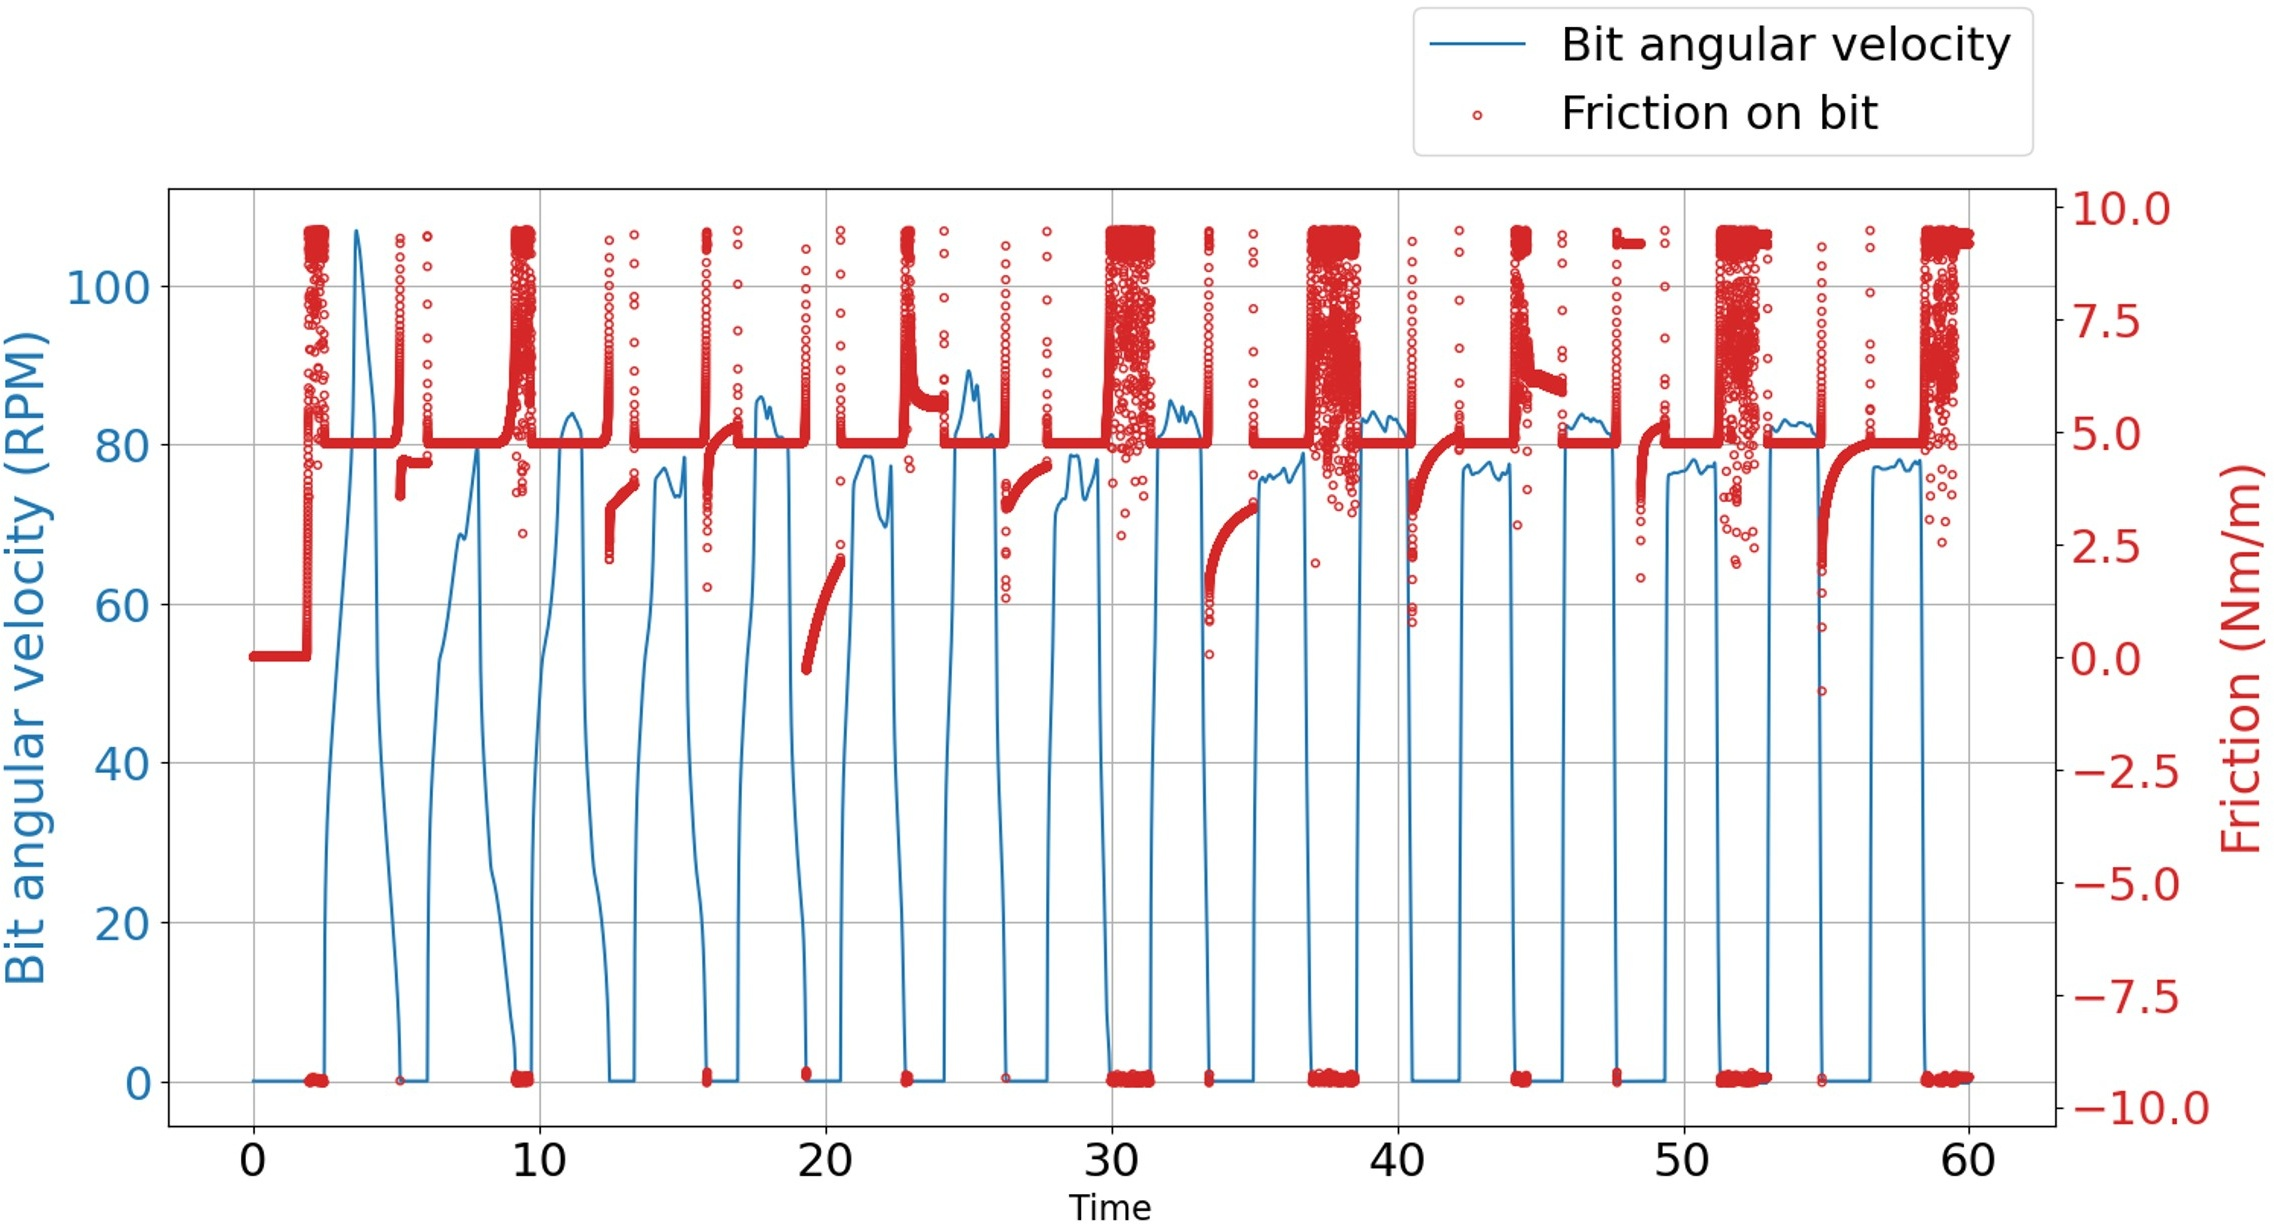
\includegraphics[width=0.85\linewidth]{friction_at_bit_stribeck_time}
			\subcaption{The frictional force at the bit and the angular velocity from the A-S drill string model using a Stribeck friction model.}
			\label{fig:friction_at_bit_stribeck_time}
		\end{minipage}
	\end{minipage}
    \caption[The friction forces from the A-S drill string model using a Stribeck friction model]{The friction forces from the A-S drill string model using a Stribeck friction model.  In~(\subref{fig:friction_at_bit_stribeck_hysteresis}), the calculated results are compared to be Coulomb and Stribeck friction models.  In~(\subref{fig:friction_at_bit_stribeck_time}), the calculated friction force is compared to the bit angular velocity.}
    \label{fig:friction_at_bit_stribeck}
\end{figure}

\begin{figure}
	\centering
	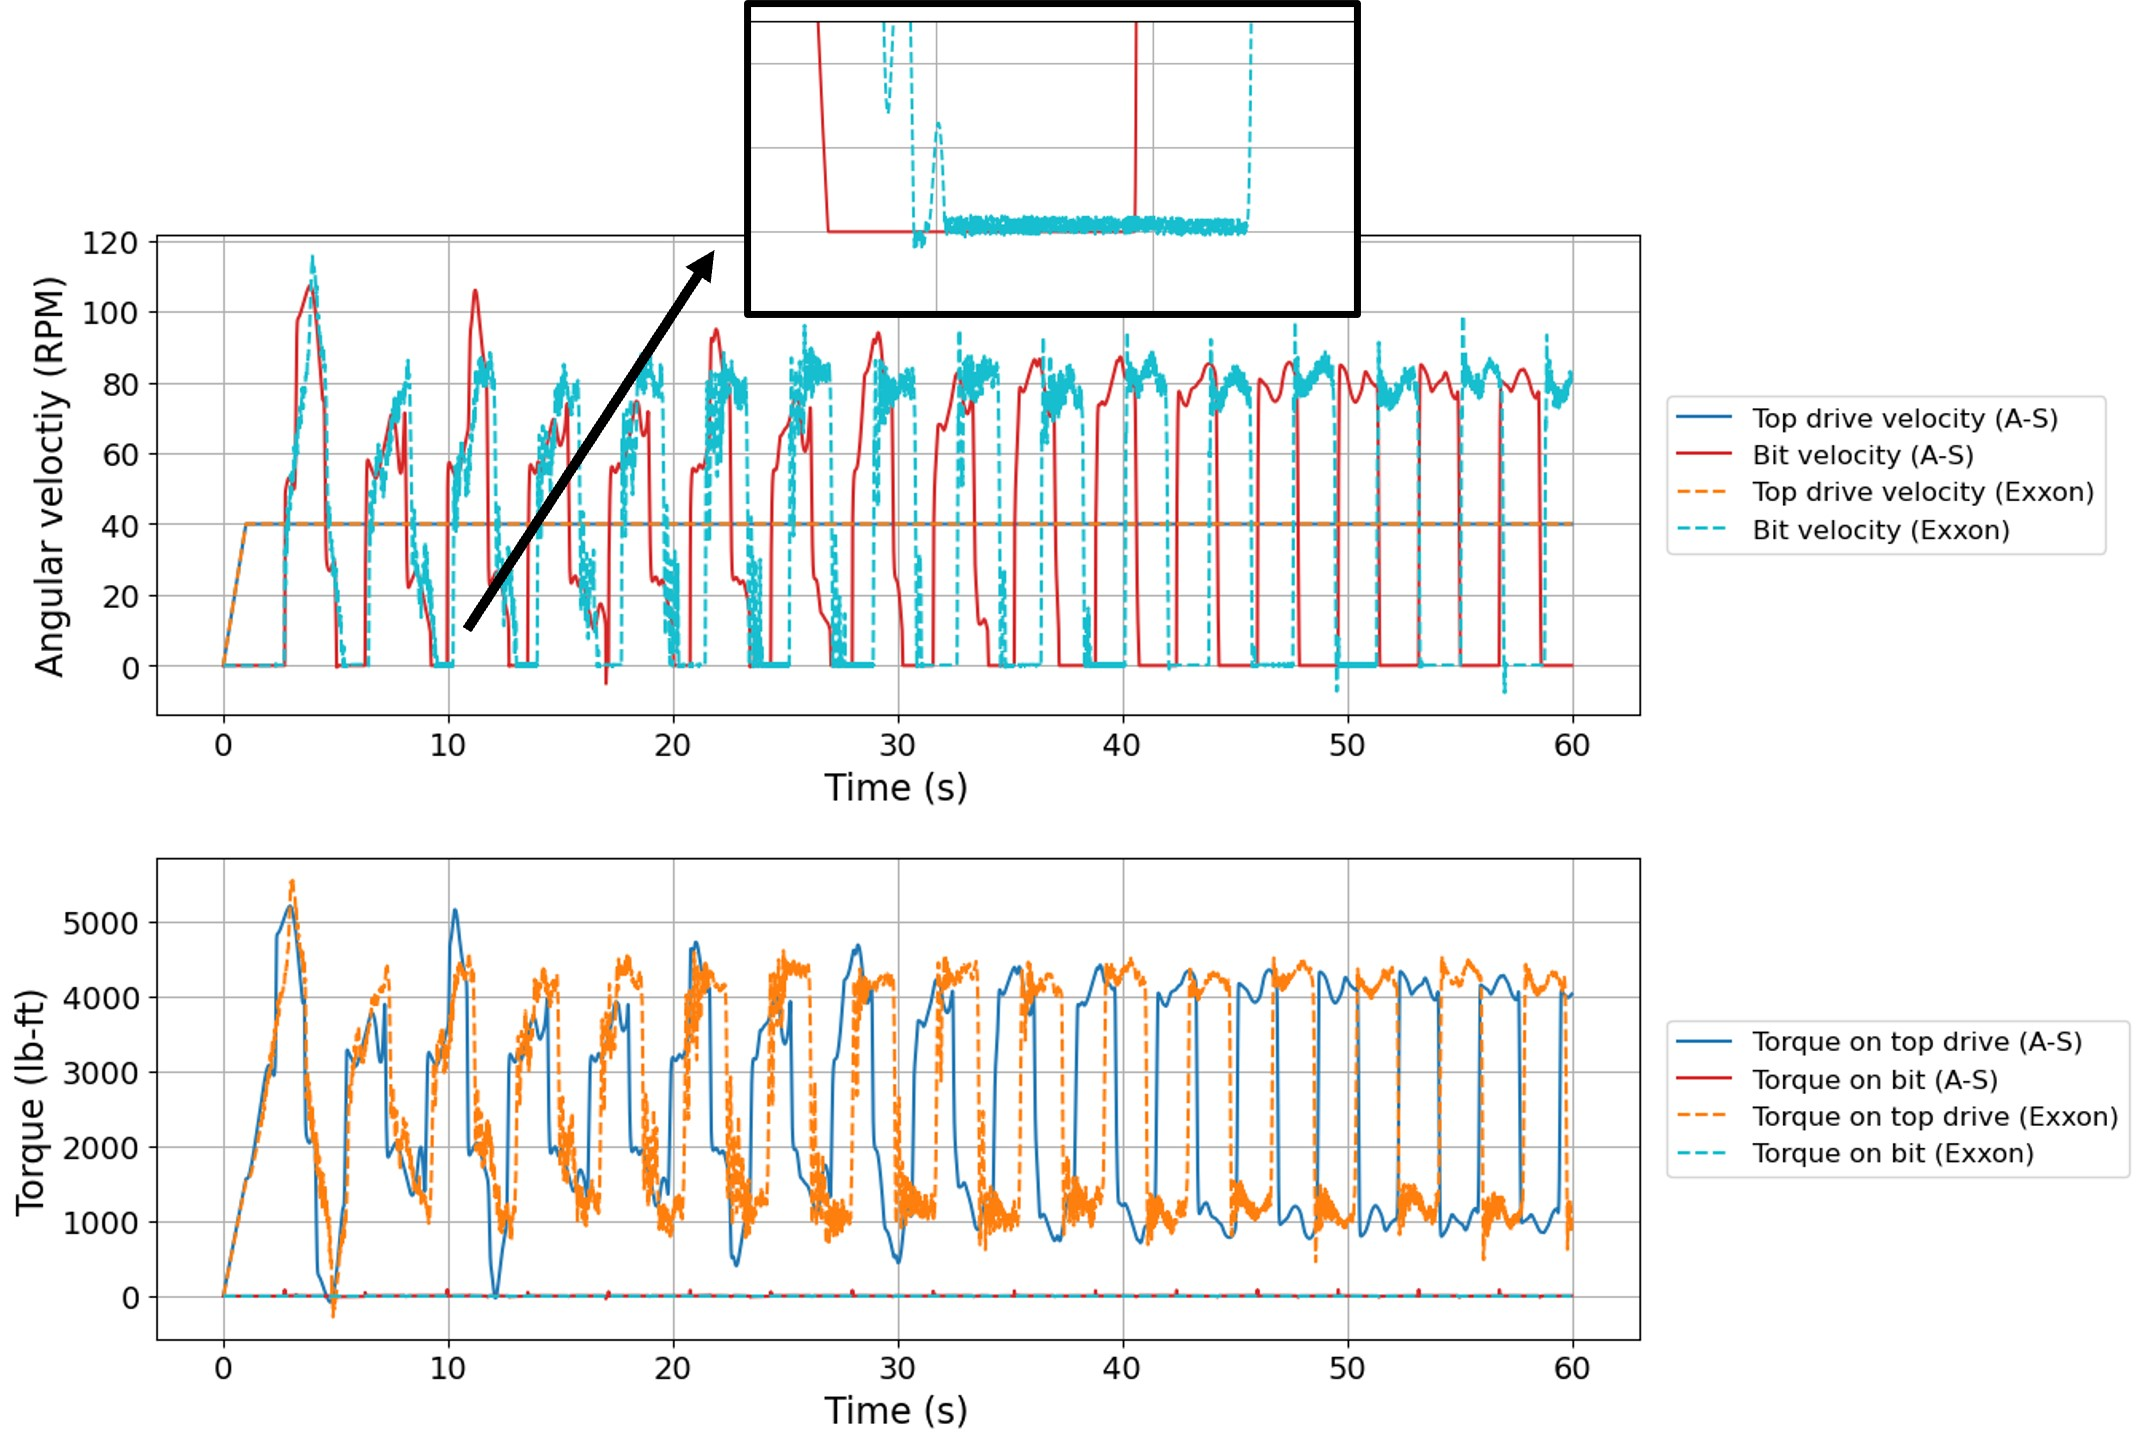
\includegraphics[width=\linewidth]{friction_comp_coulomb_stribeck}
    \caption[Comparison between A-S (Coulomb friction) and ExxonMobil (Stribeck friction) model.]{Comparison between A-S (Coulomb friction) and ExxonMobil (Stribeck) model. The fluctuation of the bit angular velocity is only observed from ExxonMobil model.}\label{figure_coloumb_coulomb}
\end{figure}

\begin{figure}
	\centering
	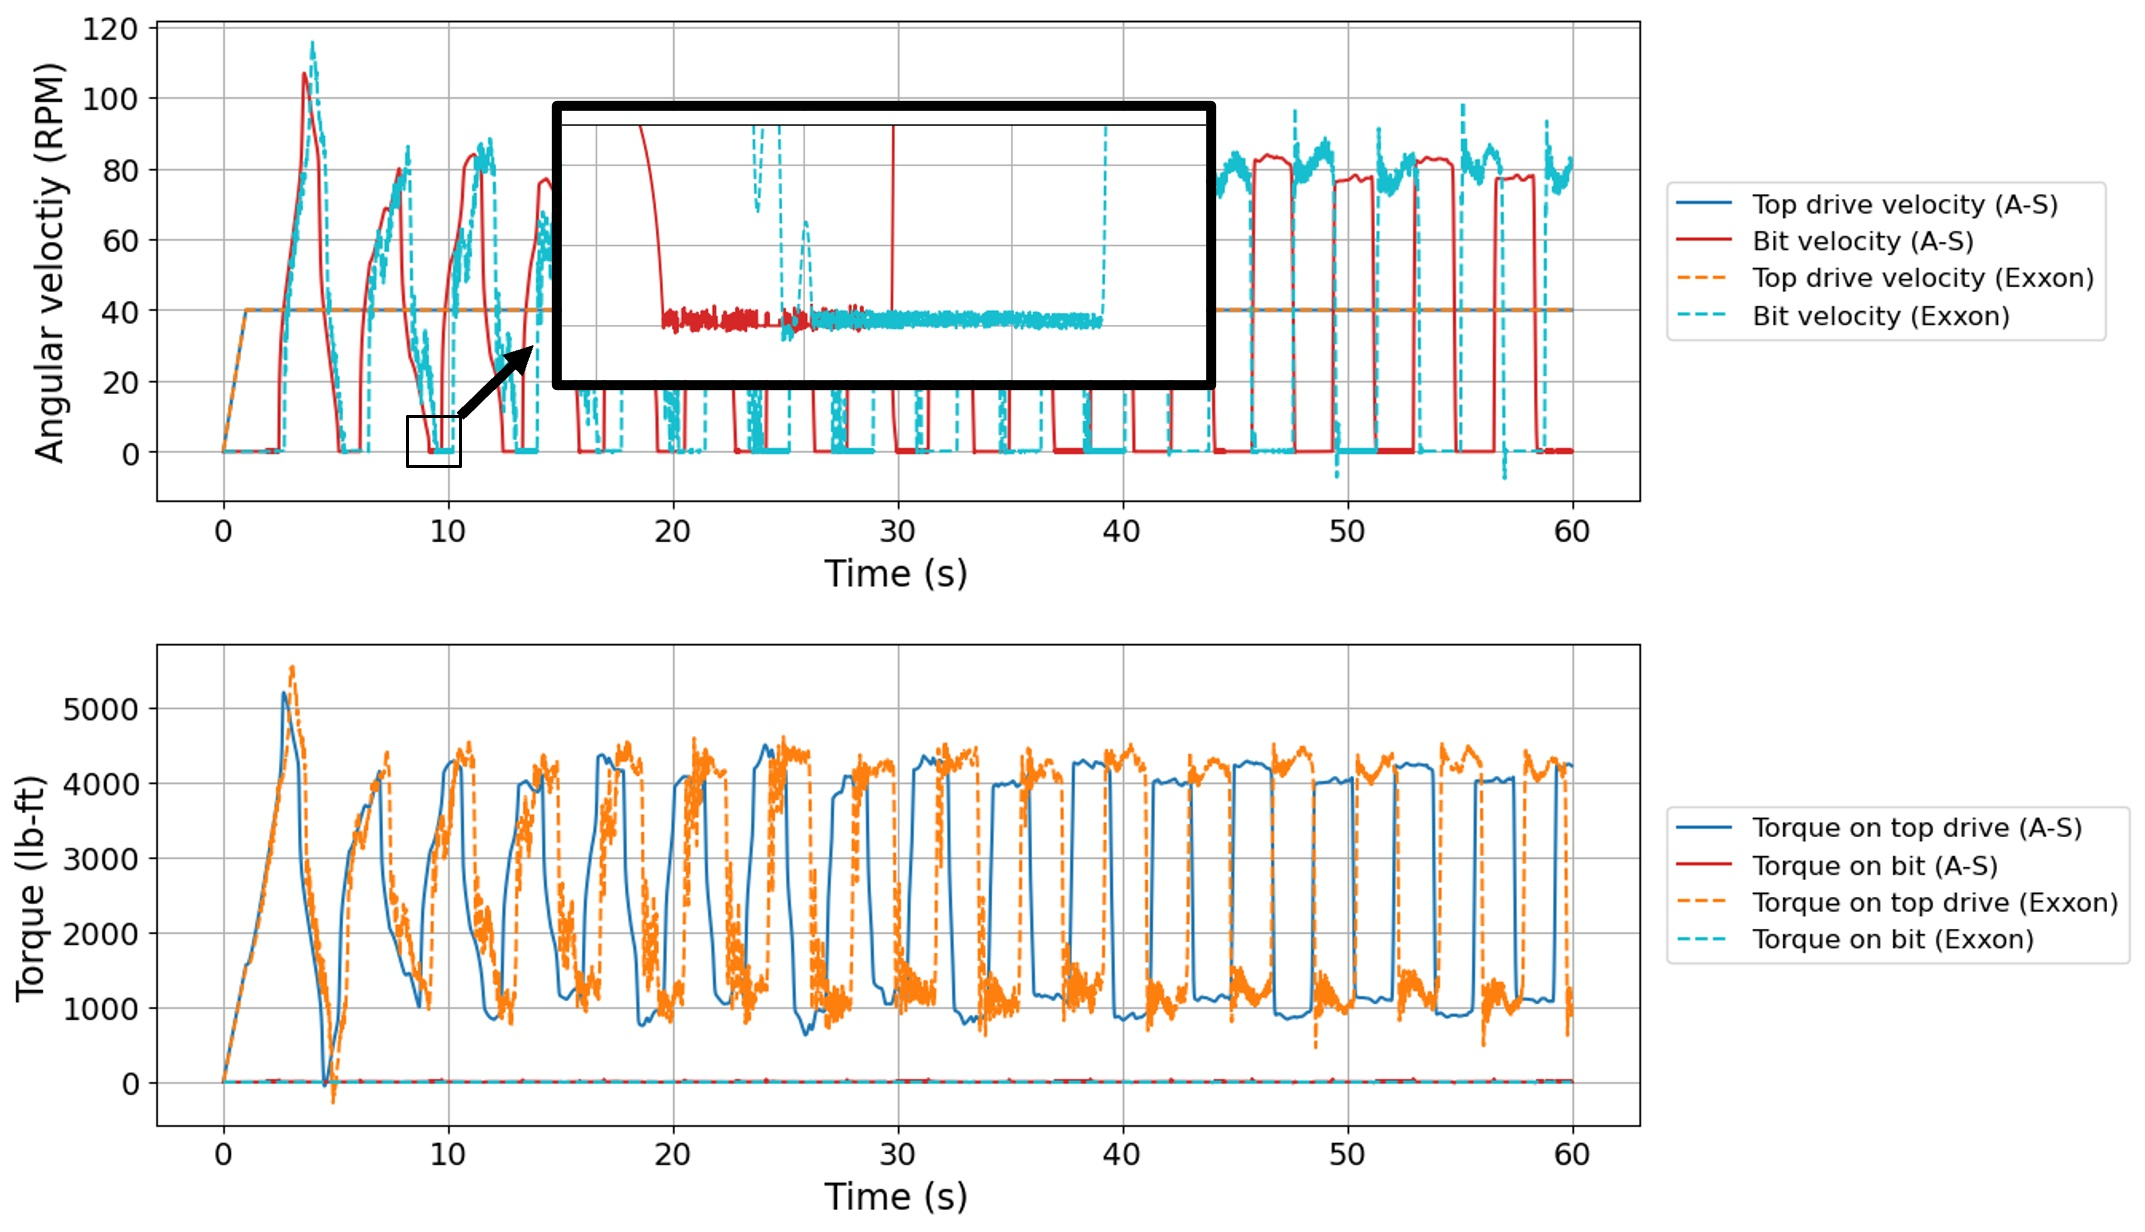
\includegraphics[width=\linewidth]{friction_comp_stribeck_stribeck}
    \caption[Comparison between A-S (Stribeck friction) and ExxonMobil (Stribeck friction) model.]{Comparison between A-S (Stribeck friction) and ExxonMobil (Stribeck) model. The fluctuation of the bit angular velocity are observed from both models.}
    \label{figure_coulomb_stribeck}
\end{figure}

